\section{Protocol and Design Rationale}
\label{sec:protocol}

The protocol runs in \emph{epochs}. An epoch $\mathtt{eid}$ deals a pool of $\Kmax$ independent keys $P_0, \dots, P_{\Kmax-1}$; each application registered against it claims one key. Operators hold registered share-encryption keys $\mathsf{pub}_i$ (\S\ref{sec:impl}); admission is a deployment concern. On the block axis an epoch passes a selection window, a contribution window and a key-assembly gap, then stays $\textsc{Live}$ with all $\Kmax$ keys stored.

\subsection{Committee Selection}
\label{subsec:lottery}

The initiator submits $(t, n, m_{\min}, \alpha)$ (threshold, committee size, minimum accepted contributions, oversubscription) and the contract snapshots the number $N$ of active operators, pins a seed block $b_s$ a few blocks ahead and stores $\tau := \lfloor 2^{256} \alpha n / N \rfloor$. The first claim after $b_s$ freezes $\mathsf{seed} := \mathsf{blockhash}(b_s)$; operator $\mathsf{op}$ is admissible iff $\mathsf{keccak}(\mathsf{seed} \,\|\, \mathsf{op}) < \tau$, and the first $n$ admissible claimants take the slots; only operators active before creation may claim. This is snapshot-based \emph{eligibility filtering}, not an unbiasable sampler: the seed's proposer can resample or withhold it, and inclusion latency decides among admissible claimants; \S\ref{sec:security} assumes the selected committee meets the corruption bound.

Epochs are created permissionlessly once $\mathsf{EPOCH\_DURATION}$ blocks have elapsed, or earlier once the newest epoch is $\textsc{Live}$ with at most one unclaimed key or aborted; deployment immutables floor $t$ and $n$ and cap $\alpha$, which a creation-race winner can pin every epoch to. Robustness depends on the chosen epoch's $n - t$: the floors enforce no margin, since $t = n$ is admissible, so tolerating $r$ unavailable members needs $t \le n - r$.

\subsection{Epoch Key Generation}
\label{subsec:epoch}

\paragraph{Contribution.} Each member $i$ samples, for every key $j$, $0 \le j < \Kmax$, a uniform polynomial $f_i^{(j)}(x) := \sum_{k<t} a_{i,j,k}\, x^k$ over $\FB_q$ and one nonce $r_{i,u}$ per recipient $u$, and publishes in one transaction the commitments $C_i^{(j)}(k) := a_{i,j,k}\, G$ and, for every $(j, u)$, the encrypted share
\[
    E_i^{(j)}(u) := \big(R_i(u), \sigma_i^{(j)}(u)\big)
    = \big(r_{i,u} G,\ f_i^{(j)}(u) + \HP(\mathsf{ctx}_{i,u} \| j \| r_{i,u} \mathsf{pub}_u) \bmod q\big)
\]
and a proof $\pi_i$ that \eqref{eq:feldman} holds and every $E_i^{(j)}(u)$ encrypts $f_i^{(j)}(u)$ (\S\ref{sec:succinct}). The commitments are digested per key, and the $\Kmax$ digests again into a single $\mathtt{commitmentsHash}$, which the contract stores after verifying $\pi_i$; the shares stay in calldata, whose $\Kmax(2t+n) + 5n$ words are sized by the epoch's $(t, n)$, not by the circuit's capacity (\S\ref{subsec:compact}). By Lemma~\ref{lem:dealing} an accepted contribution is a correct dealing to all $n$ recipients, so no complaint phase \cite{pedersen1991threshold,gennaro1999secure} is needed.

\paragraph{Finalization.} Let $A_j := \sum_{\ell \in \QUAL} f_\ell^{(j)}$, $\Cbar^{(j)}(k) := \sum_{\ell \in \QUAL} C_\ell^{(j)}(k)$, $P_j := \Cbar^{(j)}(0) = A_j(0)\,G$ and $D_{j,i} := \sum_{k<t} i^k\, \Cbar^{(j)}(k) = A_j(i)\,G$ for $i \in [n]$. After the contribution window, with at least $m_{\min}$ accepted contributions and the key-assembly gap elapsed, anyone may call $\mathsf{finalizeEpoch}$, with no deadline, carrying one proof for the whole pool: that the $\Cbar^{(j)}(k)$ aggregate the commitments of the transcript's dealer rows for every key $j$ and that the $D_{j,i}$ are the evaluations at every committee position (\S\ref{sec:succinct}). The rows are not the finalizer's choice: the contract requires them to be exactly the accepted set it recorded---$|\QUAL|$ distinct indices in $[n]$, each an accepted contributor with its stored $\mathtt{commitmentsHash}$, every inactive row zero---so $\QUAL$ is determined by the contract, never by a prover picking a subset. In one transaction the contract freezes $\QUAL$, stores every $P_j$ and $\mroot{j}$, a Keccak Merkle root over $\Nmax$ tagged leaves $\mathsf{keccak}(\mathtt{0x00} \,\|\, D_{j,i})$, $i \le n$, a constant empty leaf beyond $n$ and inner nodes $\mathsf{keccak}(\mathtt{0x01} \,\|\, l \,\|\, r)$, and marks the epoch $\textsc{Live}$; there is no per-key activation step. Our test deployment uses a $100$-block selection window, a $150$-block contribution window, a $10$-block gap and a $7\,200$-block epoch cadence; members attempt finalization in seed-derived stagger slots, so normally one node proves and a later one finds the epoch live. An epoch short of its committee or its $m_{\min}$ rows is dead. Every member $i \in [n]$ obtains $e_{j,i} := A_j(i)$ by decrypting the calldata, whether or not it dealt: decryption tolerates $n - t$ absent members.

\subsection{Applications and Their Keys}
\label{subsec:apps}

Registration against a $\textsc{Live}$ epoch names a non-zero field element $\mathtt{aid}$ and a policy, and claims the next unclaimed key $P_j$; every key of a live epoch is usable, so it fails only once the pool is exhausted. In the \emph{organizer-locked} mode the registrant, the organizer, also submits $\mathsf{PK}_{\mathtt{org}} = \mathsf{sk}_{\mathtt{org}} G$ with a Schnorr proof of possession $(A, z) = (wG,\ w + c\,\mathsf{sk}_{\mathtt{org}})$, where $c := \HK(\mathsf{dom}_{\mathtt{org}} \| \mathtt{eid} \| \mathtt{aid} \|\allowbreak \mathsf{PK}_{\mathtt{org}} \| A)$, checked as $zG = A + c\,\mathsf{PK}_{\mathtt{org}}$; it excludes rogue keys such as $-P_j$. The application key is $\mathsf{PK}_{\mathtt{aid}} := P_j + \mathsf{PK}_{\mathtt{org}}$. In the \emph{automatic} mode there is no organizer key: the contract records the identity and $0$, $\mathsf{PK}_{\mathtt{aid}} := P_j$, and any $t$ share holders decrypt.

A user encrypts $m$ as $(C_1, C_2) := (rG,\; mG + r\,\mathsf{PK}_{\mathtt{aid}})$, $r \leftarrow \FB_q$: exponential ElGamal, additively homomorphic, $m$ being recovered from $mG$ by a bounded search. Since every key is dealt by independent polynomials, the committee's term $A_j(0)\,C_1$ is useless under any other application's key (Theorems~\ref{thm:automatic} and~\ref{thm:locked}).

\paragraph{Policy.} Registration fixes who may submit (anyone, an allow-list or the registrant), a submission block window and a decryption window. Ciphertexts are accepted only inside the submission window and before decryption closes; partials and combines only inside the decryption window and, for a locked application, after the reveal. Honest nodes (fewer than $t$ corrupt) release no partial before this gate opens (\S\ref{sec:limits}).

\subsection{Threshold Decryption}
\label{subsec:decryption}

% Decryption of one ciphertext: submit, optional reveal (locked applications only),
% threshold partials, combine. Every arrow into the contract is a transaction.
\begin{figure}[t]
\centering
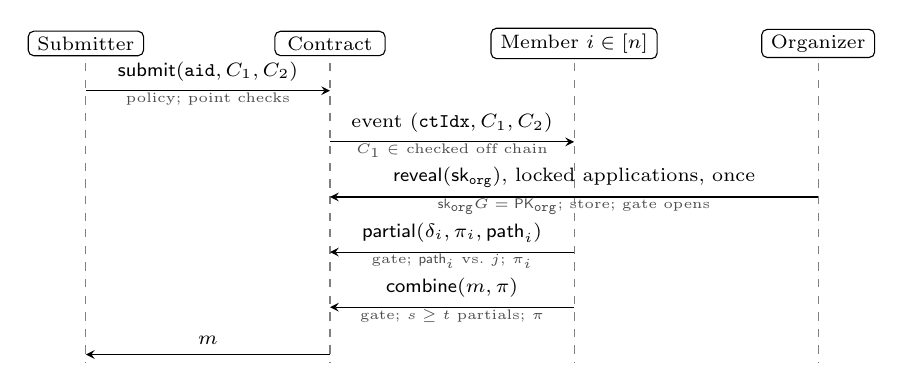
\begin{tikzpicture}[font=\scriptsize, >=stealth, note/.style={inner sep=0.5pt, font=\tiny, text=black!70}]
  \def\colS{0} \def\colC{3.1} \def\colM{6.2} \def\colO{9.3}
  \foreach \x/\n in {\colS/Submitter, \colC/Contract, \colM/Member $i \in [n]$, \colO/Organizer} {
    \node[draw, rounded corners=2pt, minimum width=1.4cm, inner ysep=2pt] at (\x,0) {\n};
    \draw[dashed, gray] (\x,-0.25) -- (\x,-4.05);
  }
  \draw[->] (\colS,-0.6) -- node[above] {$\mathsf{submit}(\mathtt{aid}, C_1, C_2)$}
    node[below, note] {policy; point checks} (\colC,-0.6);
  \draw[->] (\colC,-1.25) -- node[above] {event $(\mathtt{ctIdx}, C_1, C_2)$}
    node[below, note] {$C_1 \in \GC$ checked off chain} (\colM,-1.25);
  \draw[->] (\colO,-1.95) -- node[above] {$\mathsf{reveal}(\mathsf{sk}_{\mathtt{org}})$, locked applications, once}
    node[below, note] {$\mathsf{sk}_{\mathtt{org}} G = \mathsf{PK}_{\mathtt{org}}$; store; gate opens} (\colC,-1.95);
  \draw[->] (\colM,-2.65) -- node[above] {$\mathsf{partial}(\delta_i, \pi_i, \mathsf{path}_i)$}
    node[below, note] {gate; $\mathsf{path}_i$ vs.\ $\mroot{j}$; $\pi_i$} (\colC,-2.65);
  \draw[->] (\colM,-3.35) -- node[above] {$\mathsf{combine}(m, \pi)$}
    node[below, note] {gate; $s \ge t$ partials; $\pi$} (\colC,-3.35);
  \draw[->] (\colC,-3.95) -- node[above] {$m$} (\colS,-3.95);
\end{tikzpicture}
\caption{Decryption of a ciphertext on pool key $P_j$; arrows into the contract are transactions. Partials and the combine carry Groth16 proofs, partials also a Merkle path for $D_{j,i}$; the gate is the decryption window plus, for locked applications, the one-shot reveal.}
\label{fig:decryption}
\end{figure}


\paragraph{Submission.} $\mathsf{submitCiphertext}(\mathtt{aid}, C_1, C_2)$ carries no proof (Figure~\ref{fig:decryption}): the contract enforces the policy, assigns $\mathtt{ctIdx}$ on chain and checks both points well formed and not the identity, leaving the prime-order check to the member about to multiply its share into $C_1$, since a cofactor component would leak $e_{j,i} \bmod 8$ through its partial.

\paragraph{Partial decryption.} Any member $i \in [n]$ publishes $\delta_i := e_{j,i} C_1$ with a DLEQ proof \cite{chaum1992wallet} $(A_i, B_i, z_i) := (w_i G,\ w_i C_1,\ w_i + c_i\, e_{j,i})$, $w_i \leftarrow \FB_q$, with challenge $c_i := \HP(\mathsf{dom} \| \mathtt{eid} \| \mathtt{aid} \| \mathtt{ctIdx} \| i \|\allowbreak D_{j,i} \| C_1 \| \delta_i \| A_i \| B_i)$, verified as $z_i G = A_i + c_i D_{j,i}$ and $z_i C_1 = B_i + c_i\,\delta_i$ inside a Groth16 proof $\psi_i$ (\S\ref{sec:succinct}), and a Merkle path for $D_{j,i}$ that the contract checks against $\mroot{j}$ at leaf $i - 1$.

\paragraph{Reveal.} A locked application's organizer publishes $\mathsf{sk}_{\mathtt{org}}$ through the permissionless, one-shot $\mathsf{revealOrganizerSecret}$ call; the contract checks $\mathsf{sk}_{\mathtt{org}} G = \mathsf{PK}_{\mathtt{org}}$ and stores it. Until then no partial or combine of the application exists on chain; afterwards every past and future ciphertext is eligible, so the organizer decides \emph{when}, not \emph{which} (\S\ref{sec:limits}).

\paragraph{Combine.} Once $s \ge t$ partials from $\QC = \{x_1, \dots, x_s\}$ are on chain and the gate is open, anyone submits a proof establishing, with the canonical Lagrange coefficients $\lambda_k$ of $\QC$ (\S\ref{sec:succinct}),
\begin{align}
    \sum_{k} \lambda_k\, \delta_{x_k} = A_j(0)\, C_1, \qquad
    M = C_2 - \sum_k \lambda_k\, \delta_{x_k} - \mathsf{sk}_{\mathtt{org}}\, C_1 = mG,
    \label{eq:combine}
\end{align}
and, from the private witness $\mathsf{sk}_{\mathtt{org}}$, that $\mathsf{sk}_{\mathtt{org}} G$ is the $\mathsf{PK}_{\mathtt{org}}$ on record, trivially for an automatic application. The combiner recovers $m$ off chain by baby-step giant-step \cite{shanks1971class} (\S\ref{sec:impl}).

\paragraph{Design rationale.} Clients already produce exponential ElGamal ciphertexts and homomorphic aggregates, the organizer runs no prover, and the DKG verifies nothing application-specific. A proof of knowledge of $r$ with $C_1 = rG$ \cite{shoup2002threshold} is unavailable, since an aggregate's submitter does not know $\sum_k r_k$; the committee therefore answers any $C_1$ under any key it serves, so separation cannot come from a public additive offset ($\mathsf{PK}_{\mathtt{ep}} + \HK(\mathtt{aid})\,G$ \cite{bip32} is removed by shifting $C_2$ by $\HK(\mathtt{aid})\,C_1$) but only from independently dealt keys, pooled at one transaction and proof per member plus one finalization proof per epoch.
